% Бүлэг 4

\chapter{Системийн хөгжүүлэлт}
\label{Chapter4}

\section{Хөгжүүлэлтийн орчин ба технологи}
\label{sec:dev-environment}

LexNavigator системийг хөгжүүлэхдээ орчин үеийн, өндөр гүйцэтгэлтэй технологиудыг сонгосон. Гол технологиуд:
\begin{itemize}
    \item \textbf{Backend:} FastAPI + Uvicorn
    \item \textbf{Өгөгдлийн сан:} PostgreSQL (Neon) + SQLAlchemy 2.0 + Alembic
    \item \textbf{Аюулгүй байдал:} JWT + bcrypt
    \item \textbf{AI:} Google Gemini 2.5 Flash
    \item \textbf{Баримт бичиг задлах:} PyMuPDF + regex parser
\end{itemize}

\section{Модуль ба бүрэлдэхүүн хэсгүүд}

Систем нь дараах үндсэн модулиудаас бүрдэнэ:
\begin{itemize}
    \item Auth Module
    \item Chat Module
    \item Retrieval Module
    \item AI Orchestrator
    \item Data Processing Module
\end{itemize}

\begin{figure}[H]
	\centering
	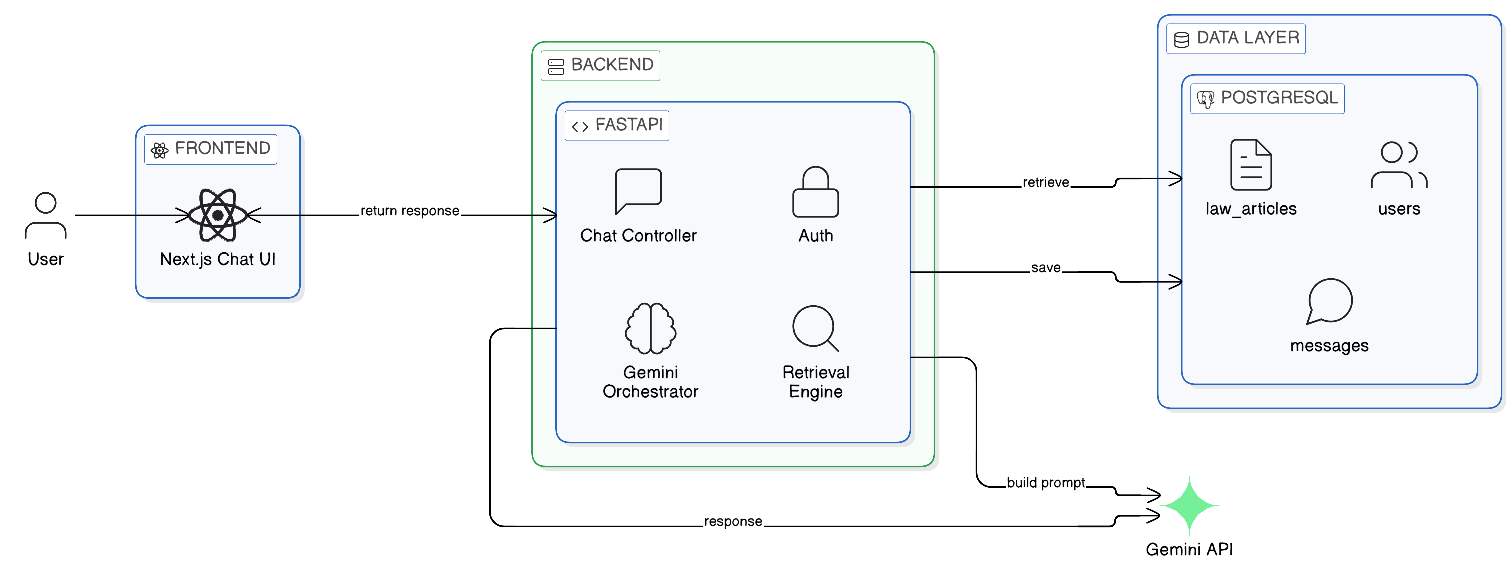
\includegraphics[width=\textwidth]{./Diagrams/SystemArchitecture.png}
	\caption{Системийн ерөнхий архитектур}
	\label{fig:ArchitectureDiagram}
\end{figure}

\section{API болон өгөгдөл солилцоо}

Гол endpoint-ууд:
\begin{itemize}
    \item \texttt{POST /api/auth/register}
    \item \texttt{POST /api/auth/login}
    \item \texttt{POST /api/chat/message}
\end{itemize}

\section{Аюулгүй байдал ба нэвтрэлт}
\label{sec:security}

Системийн аюулгүй байдлыг хангахад онцгой анхаарсан. Хэрэглэгчийн нууц үгийг хамгаалахын тулд \texttt{app/core/security.py} файлд \textbf{passlib} сангийн \texttt{CryptContext} ашиглан bcrypt hashing хийдэг.

\textbf{Нууц үгийн hashing механизм:}
\begin{itemize}
    \item \texttt{CryptContext(schemes=["bcrypt"], deprecated="auto")} ашигласан
    \item Шинэ хэрэглэгч бүртгүүлэх үед нууц үгийг автоматаар hash хэлбэрээр хадгална
    \item Нэвтрэх үед оруулсан нууц үгийг hash-тай харьцуулан шалгана
    \item bcrypt алгоритм нь brute-force халдлагад тэсвэртэй, салт (salt) автоматаар үүсгэдэг
\end{itemize}

\begin{figure}[H]
	\centering
	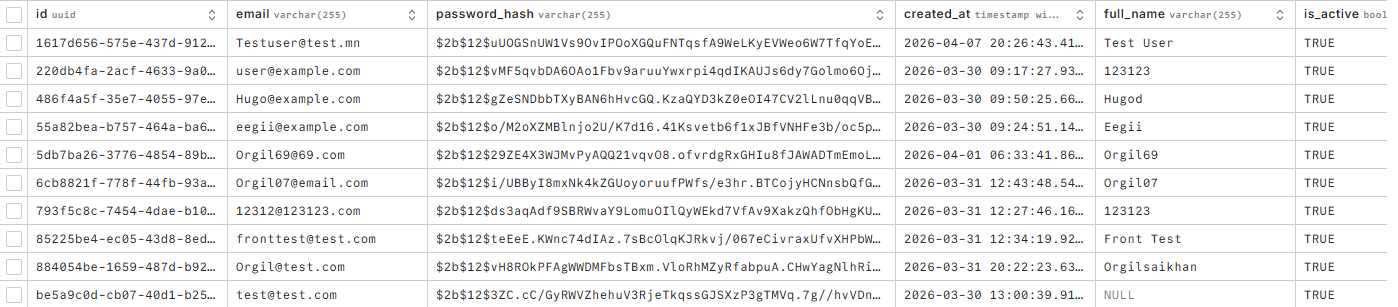
\includegraphics[width=\textwidth]{./TestPic/UserTableHash.png}
	\caption{Хэрэглэгчийн хүснэгтэд нууц үг hashing хийгдсэн байдал (bcrypt)}
	\label{fig:UserTableHashing}
\end{figure}

Нэмэлт аюулгүй байдлын шийдлүүд:
\begin{itemize}
    \item JWT токен ашиглан stateless authentication
    \item Role-based access control (user, lawyer, admin)
    \item Pydantic ашиглан input validation (SQL injection, XSS хамгаалалт)
    \item CORS middleware + HTTPS шаардлагатай
    \item API key болон database тохиргоог .env файлаар удирдана
\end{itemize}

\section{AI интеграцчилал (Gemini + RAG)}

RAG загварын урсгалыг дээрх зурагт үзүүлэв. Хэрэглэгчийн асуултыг эхлээд өгөгдлийн сангаас хайж, олдсон хуулийн заалтуудыг context болгон Gemini руу илгээдэг.

\begin{figure}[H]
	\centering
	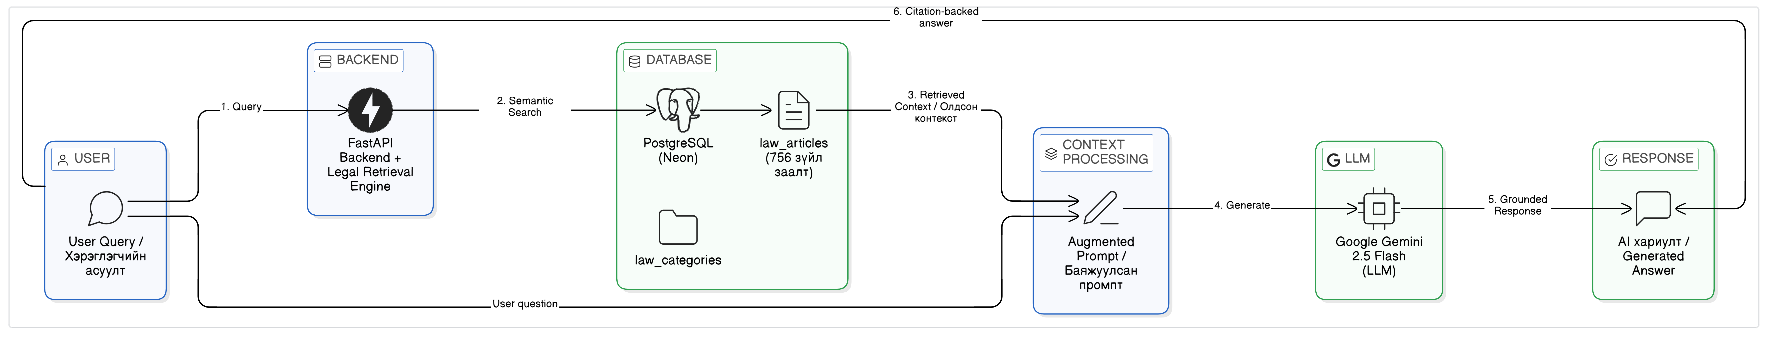
\includegraphics[width=\textwidth]{./Diagrams/RAG_Diagram.png}
	\caption{RAG (Retrieval-Augmented Generation) урсгал}
	\label{fig:RAGDiagram}
\end{figure}

\section{Хэрэгжүүлэлт (Implementation)}
\label{sec:implementation}

Системийн гол функцүүдийг амжилттай хэрэгжүүлж, Postman-ээр туршилт хийсэн. Доорх зургуудад үндсэн API endpoint-үүдийн ажиллагааг харуулав.

\subsection{Хэрэглэгчийн бүртгэл (Register)}

\begin{figure}[H]
	\centering
	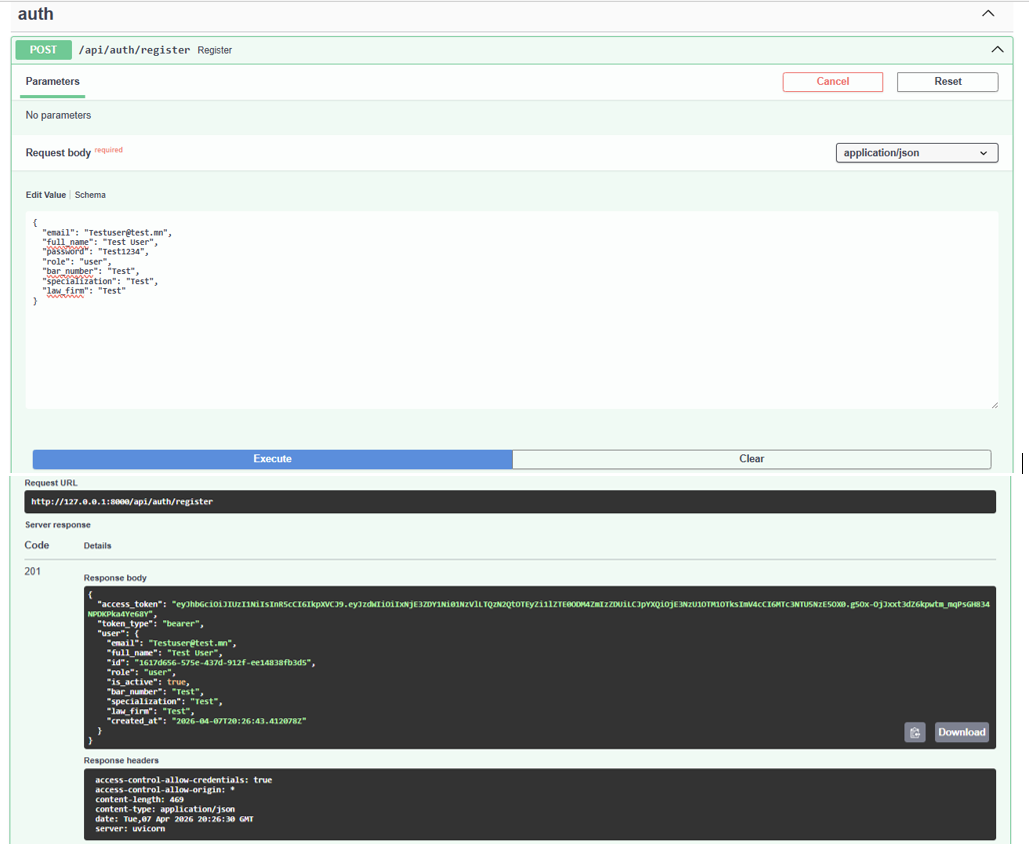
\includegraphics[width=\textwidth]{TestPic/authRegisterTest.png}
	\caption{POST /api/auth/register endpoint-ийн туршилт}
	\label{fig:RegisterTest}
\end{figure}

\subsection{Нэвтрэлт (Login)}

\begin{figure}[H]
	\centering
	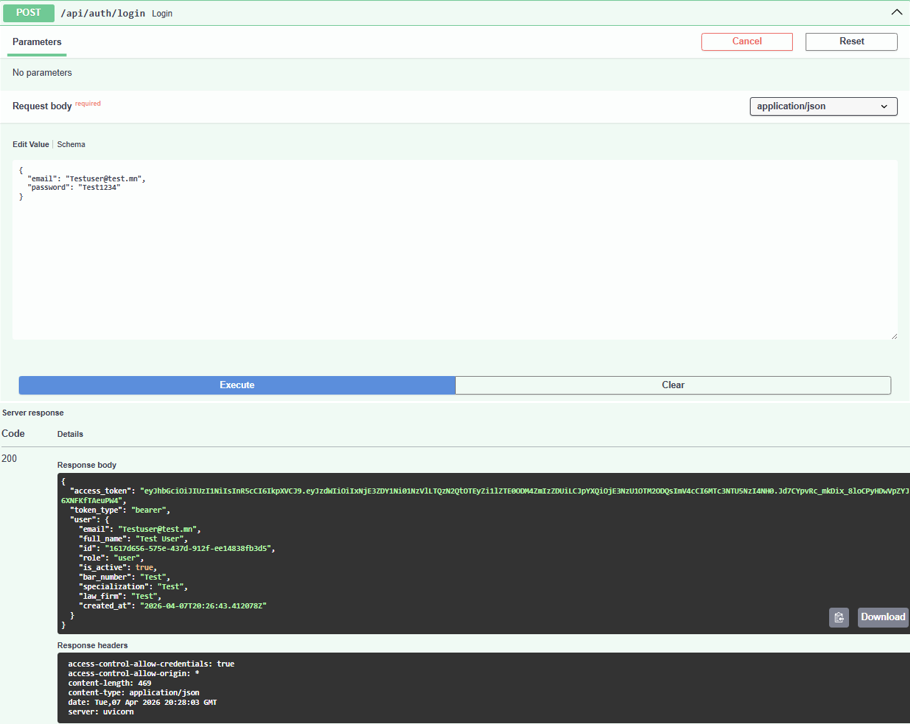
\includegraphics[width=\textwidth]{TestPic/authloginTest.png}
	\caption{POST /api/auth/login endpoint-ийн туршилт}
	\label{fig:LoginTest}
\end{figure}

\subsection{Чат мессеж илгээх ба AI хариулт авах}

\begin{figure}[H]
	\centering
	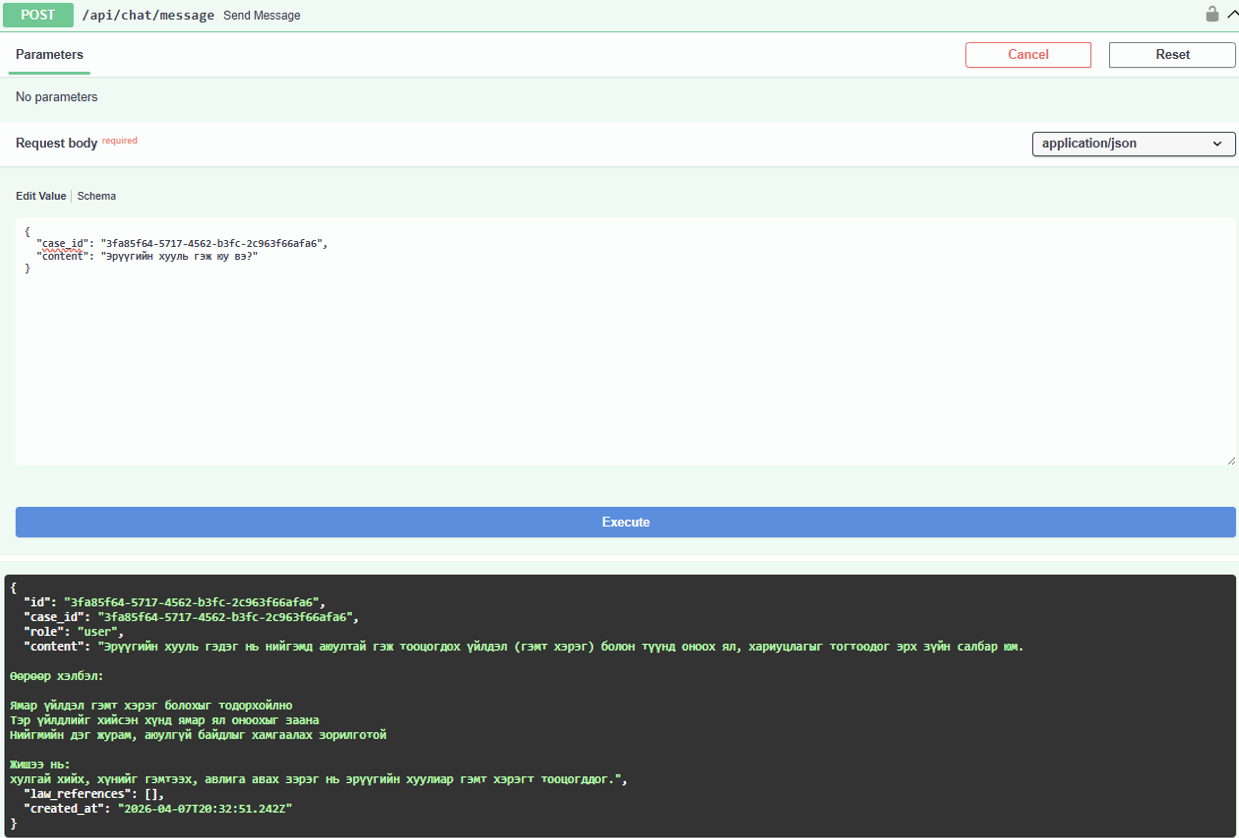
\includegraphics[width=\textwidth]{TestPic/authMessageTest.png}
	\caption{POST /api/chat/message endpoint-ийн туршилт (Монгол хэл дээр асуулт илгээж, AI хариулт авсан байдал)}
	\label{fig:MessageTest}
\end{figure}

Эдгээр туршилтаас харахад Auth, Chat модулиуд зөв ажиллаж, JWT токен амжилттай үүсэж, Gemini-ээр боловсруулсан хариулт буцаж ирж байгааг баталж байна.

\section{Бүлгийн дүгнэлт}

Энэ бүлэгт LexNavigator системийн хөгжүүлэлтийн орчин, архитектур, модульчлал, API, аюулгүй байдал, Gemini + RAG интеграцчилал болон бодит хэрэгжүүлэлтийг (Postman туршилтын зургуудтай) харуулав. Системийн үндсэн функцүүд амжилттай хэрэгжиж, цаашдын туршилт, өргөтгөл хийхэд бэлэн болсон.
